The project is implemented primarily in Python, chosen for its dominance in the \gls{ML} ecosystem and its compatibility across all services within the system architecture. The frontend is implemented in TypeScript using the Next.js framework. 

Development is conducted using Visual Studio Code as \gls{IDE}, while GitHub is employed for version control. The entire system is containerised using Docker and orchestrated with Docker Compose, enabling reproducible deployments across different host environments.

The implementation is organised into three main modules following the architecture described in \nameref{sec:proposal:design}:

\begin{itemize}
    \item \textbf{\nameref{sec:impl:frontend}}: The web application through which operators interact with the platform and monitor the device fleet.
    \item \textbf{\nameref{sec:impl:platform}}: The server-side backend responsible for device fleet management, the \gls{AI} model lifecycle, hardware compilation, and \gls{OTA} deployment orchestration.
    \item \textbf{\nameref{sec:impl:edge}}: The software stack running inside a Docker container on each physical \gls{IoT} device, handling real-time inference, telemetry, \gls{OTA} updates, and script execution.
\end{itemize}

\subsection{User Interface}\label{sec:impl:frontend}

The User Interface is implemented with Next.js and React, using TypeScript throughout. It communicates with the \gls{API} Gateway via a \gls{HTTP} client that automatically injects the \gls{JWT} access token into every request. Asynchronous data fetching, caching, and automatic polling are configured with per-view refresh intervals between 8 and 15 seconds for live-data views.

The application is structured into an authentication view and six main dashboard pages: Login, Overview, Devices, Models (which consolidates models, datasets, and training triggers), Scripts, Deployments (which integrates model compilation on-demand), and Monitoring.

To maintain the focus of this chapter on implementation architecture, the visual layout, detailed view descriptions, and corresponding screen captures for each page are in \autoref{ap:ui}.

\subsection{Cloud/Server Platform}\label{sec:impl:platform}

This section details the implementation of the Cloud/Server Platform of \gls{AURA} introduced in \nameref{sec:proposal:design:cloud}.

\begin{figure}[H]
    \centering
    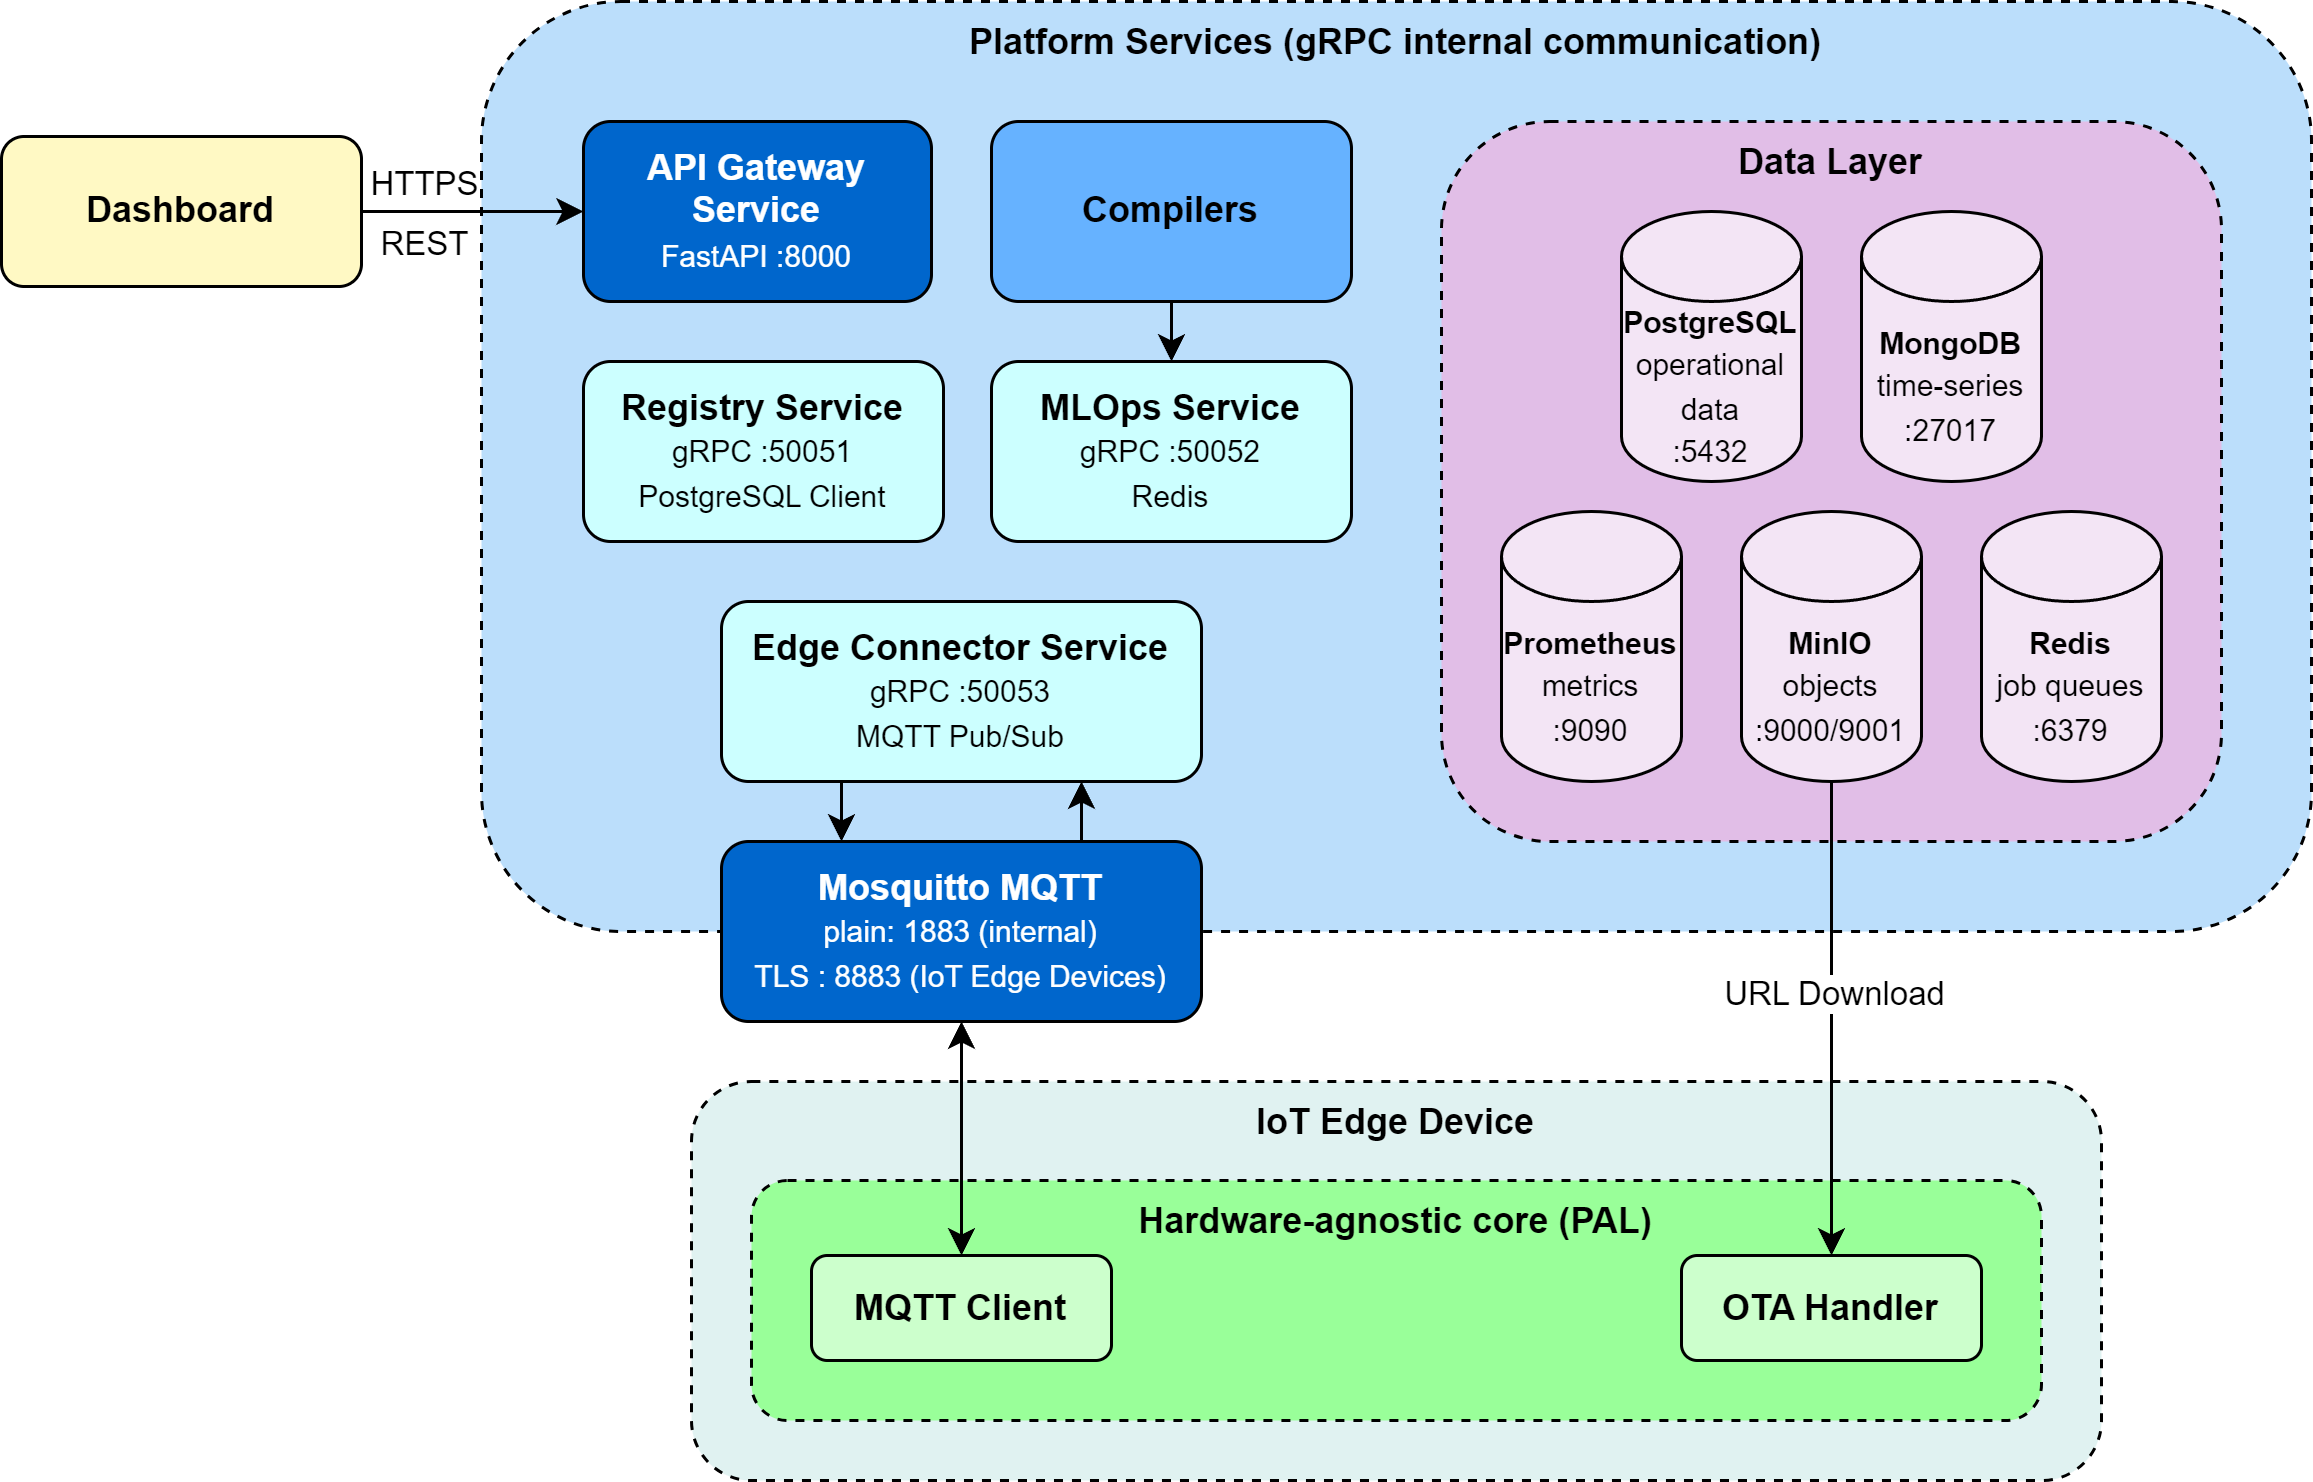
\includegraphics[width=0.97\linewidth]{images/CloudServer Platform.png}
    \caption{Cloud/Server Platform Diagram}
    \label{fig:cloud_diagram}
\end{figure}

All inter-service and service-to-database connectivity is confined to internal Docker networks, with no storage system port exposed beyond the host machine. Internal connectivity between micro-services is managed through \gls{gRPC} channels, one per downstream service. 

Communication with edge devices is routed exclusively through the Mosquitto \gls{MQTT} broker, which enforces mutual \gls{TLS} authentication on port 8883 and per-device \gls{ACL} rules that restrict each device to its own topic namespace.

\subsubsection{\texorpdfstring{\acrshort{API}}{API} Gateway}\label{sec:impl:gateway}

The \gls{API} Gateway serves as the single point of entry for all users. It is implemented with FastAPI, and listens on port 8000. Beyond request routing, it is responsible for two cross-cutting concerns: authentication and internal service connectivity.

Authentication is implemented using \glspl{JWT}. Upon successful login, the gateway issues a short-lived access token (one hour) and a refresh token (seven days), both signed with a secret key provided via environment variable. 

Subsequent requests must include the access token in the \texttt{Authorization: Bearer} header. Role-based access control enforces three privilege levels: \textit{admin}, \textit{operator}, and \textit{viewer} at the endpoint level using FastAPI dependency injection.

To handle large binary assets efficiently (such as \gls{AI} models, dataset ZIP archives, and custom scripts), the \gls{API} Gateway implements direct file upload integration with MinIO. Streaming massive binary payloads over the internal \gls{gRPC} network would introduce significant memory overhead and communication latency, 

Instead, the gateway processes multipart \gls{HTTP} requests and streams the binaries directly to their designated MinIO storage buckets. Once the file upload is successfully acknowledged, only the reference \gls{URI} and a calculated SHA-256 hash are sent to the Registry Service via \gls{gRPC} to persist the resource metadata.

The mapping between \gls{REST} routes and \gls{gRPC} services is organised into dedicated routers shown in \autoref{tab:api_routing}.

\begin{table}[H]
    \centering
    \caption{\acrshort{API} Routing and Service Mapping}
    \label{tab:api_routing}
    \begin{tabular}{p{0.18\textwidth}
                    p{0.12\textwidth}
                    p{0.20\textwidth}
                    p{0.40\textwidth}}
        \hline
        \textbf{End-Service} & \textbf{\gls{HTTP} Method} & \textbf{Endpoint} & \textbf{Description} \\
        \hline
        \textbf{\gls{API} Gateway} & \texttt{POST} & \texttt{/auth/token} & Validates credentials and refresh \glspl{JWT}. \\
        \hline
        \textbf{Registry Service} & \texttt{GET POST PUT DELETE} & \texttt{/api/devices}, \texttt{/api/models}, \texttt{/api/datasets}, \texttt{/api/scripts} & Manages device, model, dataset and script metadata, supporting retrieval, creation, update, and deletion. \\
        \hline
        \textbf{\gls{MLOps} Service} & \texttt{POST} & \texttt{/api/models/ :id/compile}, \texttt{/api/models/ train} & Queues training, retraining, and compilation tasks. \\
        \hline
        \textbf{Edge Connector} & \texttt{GET POST} & \texttt{/api/deployments} & Coordinates \gls{OTA} updates. \\
        & \texttt{GET} & \texttt{/api/monitoring/ devices}, \texttt{/api/monitoring/ inference} & Fetches real-time status and telemetry logs. \\
        \hline
    \end{tabular}
\end{table}

\subsubsection{Registry Service}\label{sec:impl:registry_svc}

The Registry Service, running on \gls{gRPC} port 50051, serves as the metadata management core of the platform. It consolidates the storage and query logic for three main domains: devices, datasets and \gls{AI} models, and custom scripts. Its implementation relies on an async SQLAlchemy session per request and a dedicated repository class for each domain.

\begin{itemize}
    \item \textbf{Device Registration}: Operators register edge nodes by providing a unique name, the target hardware type (e.g., \texttt{hailo8}), an optional text description, and lists of attached peripherals including sensors (such as cameras), actuators, and other custom components.
    
    \item \textbf{Hardware Architectures Catalog}: Associates registered devices and compiled models with their target hardware types\footnote{In this \gls{PoC}, there are five hardware architectures pre-seeded (\gls{RPi} 5 (\gls{CPU}), Hailo-8/8L, \gls{RPi} \gls{AI} Camera, and Jetson Orin Nano).}. While the Registry Service handles the persistence of these associations, the actual definitions, compilation parameters, and toolchains for each architecture are managed by the \gls{MLOps} Service (detailed in \autoref{tab:hardware_toolchains}). It is possible to add more hardware architectures manually (\autoref{sec:impl:dyn_hardware}).
    
    \item \textbf{Dataset Catalog}: Manages datasets metadata, including name, description, size in bytes, and SHA-256 hash. File uploads are coordinated with the browser: the registry registers the dataset metadata and provides coordinates for directly uploading the compressed archive to the MinIO object store.
    
    \item \textbf{\gls{AI} Model Registry}: Keeps track of both source and compiled models, as well as their lineage across training cycles. It registers the source model parameters (epochs, batch size, input size, and base YOLO architecture) and maps the model association to its corresponding dataset.
    
    \item \textbf{Scripts Catalog}: Registers custom Python processing scripts that operators write to execute with the inference on \gls{IoT} Edge devices. It saves references to the script files stored in MinIO and maintains their checksums for \gls{OTA} integrity checks.
\end{itemize}

\subsubsection{\texorpdfstring{\acrshort{MLOps}}{MLOps} Worker Service}\label{sec:impl:mlops_worker_svc}

The \gls{MLOps} Worker Service, running on \gls{gRPC} port 50052, acts as an arq worker connected to a Redis queue, consuming training, retraining and compilation tasks. It handles \gls{CPU}/\gls{GPU}-intensive tasks asynchronously to prevent blocking the \gls{API} Gateway or registry requests.

\begin{itemize}
    \item \textbf{Asynchronous Model Training}: When a training/retraining job is triggered, the worker downloads the dataset ZIP file from MinIO, extracts it, and launches the YOLO training loop. It streams execution logs (loss, accuracy, epochs) in real-time to a Redis collection to be monitored by the frontend, and uploads the resulting PyTorch model (\texttt{best.pt}) back to MinIO before notifying the Registry Service of the completion.
    
    \item \textbf{Model Compilation}: Converts generic PyTorch models to hardware-native formats. \autoref{tab:hardware_toolchains} shows the compilation toolchains, output formats, and configurations used per target in this \gls{PoC}.
\end{itemize}

\begin{table}[H]
    \centering
    \caption{Pre-seeded Hardware Architectures, Compilation Toolchains and Formats} 
    \label{tab:hardware_toolchains}
    \begin{tabular}{p{0.20\textwidth}
                    p{0.14\textwidth}
                    p{0.44\textwidth}
                    p{0.17\textwidth}}
        \hline
        \textbf{Backend \gls{ID}} & \textbf{Output Format} & \textbf{Toolchain \& Environment} & \textbf{Default Arguments} \\ \hline
        \texttt{hailo8} & \texttt{.hef} & Hailo \gls{AI} Software Suite Docker image, \texttt{hailomz compile} CLI & \texttt{\{"hw-arch": "hailo8"\}} \\
        \texttt{hailo8l} & \texttt{.hef} & Hailo \gls{AI} Software Suite Docker image, \texttt{hailomz compile} CLI & \texttt{\{"hw-arch": "hailo8l"\}} \\
        \texttt{rpi\_ai\_cam} & \texttt{network.rpk} & \texttt{imx500-converter}, Sony Model Compression Toolkit (MCT) & \texttt{\{"format": "imx"\}} \\
        \texttt{jetson\_orin\_nano} & \texttt{.engine} & CUDA and NVIDIA's TensorRT compiler container & \texttt{\{"format": "engine"\}} \\
        \texttt{rpi} & \texttt{.onnx} & PyTorch and Ultralytics native exporters & \texttt{\{"format": "onnx"\}} \\ \hline
    \end{tabular}
\end{table}

\todo{actualizar hw}

\subsubsection{Edge Connector Service}\label{sec:impl:edge_connector_svc}

The Edge Connector Service, running on \gls{gRPC} port 50053, acts as the bridge between the server-side platform and the set of \gls{IoT} Edge devices. It combines \gls{OTA} deployment orchestration, telemetry monitoring, and Prometheus metric export.

\begin{itemize}
    \item \textbf{\gls{OTA} Deployment Orchestration}: Coordinates the delivery of models and scripts to edge devices. When a deployment is requested, it ensures compilation is completed, generates short-lived presigned \glspl{URL} for MinIO assets, saves the deployment transaction with status \textit{pending}, and publishes a \texttt{deploy} command to \texttt{device/\{id\}/commands} over \gls{MQTT}. It listens to acknowledgment events on \texttt{device/+/events} to update the status in PostgreSQL from \textit{sent} to \textit{running} or \textit{failed}.
    
    \item \textbf{\gls{OTA} Library Sync}: If the device's hardware library files hash does not match the platform's current version, it packages the local hardware folder, uploads it to MinIO, and publishes an \texttt{update\_libraries} command to force the edge runtime to synchronize.
    
    \item \textbf{Telemetry \& Inference Monitoring}: Subscribes to telemetry and inference topics. Upon receiving telemetry from \texttt{device/\{id\}/telemetry}, it saves the \gls{CPU}/\gls{RAM} metrics and active deployments state to MongoDB, and updates the Prometheus metrics. 
    
    \item \textbf{Inference Storage}: Receives real-time predictions from \texttt{device/\{id\}/inference} and records them in MongoDB for historical telemetry analytics.
\end{itemize}

Communication with edge devices is routed asynchronously through the \gls{MQTT} broker using \gls{TLS}. The service subscribes to and publishes on the following device-specific topics, structured dynamically under the device identifier namespace:
\begin{itemize}
    \item \textbf{\texttt{device/\{device\_id\}/telemetry}}: Inbound topic where edge devices publish periodic health performance data (\gls{CPU}, \gls{RAM}, temperatures, and active deployment status) to update MongoDB and Prometheus metrics.
    \item \textbf{\texttt{device/\{device\_id\}/inference}}: Inbound topic where the edge Orchestrator streams real-time YOLO object detection payloads (classes, bounding boxes, and confidence levels) to be persisted in MongoDB.
    \item \textbf{\texttt{device/\{device\_id\}/events}}: Inbound topic for status events published by the edge \gls{OTA} Handler (such as \texttt{deploy\_ack}, \texttt{deploy\_failed}, or \texttt{update\_libraries\_ack}) to coordinate platform database states.
    \item \textbf{\texttt{device/\{device\_id\}/commands}}: Outbound topic where the platform publishes execution instructions (such as \texttt{deploy}) to the edge nodes.
\end{itemize}

\subsubsection{Data Layer}\label{sec:impl:data}

The five storage systems introduced in \autoref{sec:proposal:design} are implemented as follows.

\begin{itemize}
    \item \textbf{PostgreSQL} (port 5432) stores all operational metadata. The schema includes tables for \texttt{devices}, \texttt{datasets}, \texttt{models}, \texttt{scripts}, and \texttt{deployments}.
    \item \textbf{MongoDB} (port 27017) stores unstructured time-series data: the \texttt{telemetry\_history} collection registers \gls{CPU}, memory usage and device statuses, while the \texttt{inference\_results} collection stores predictions published by edge nodes.
    \item \textbf{MinIO} (port 9000) acts as the object storage. It is organised into dedicated buckets: \texttt{models} for original models, \texttt{compiled} for compiled hardware-native binaries, \texttt{datasets} for raw image packages, \texttt{base-models} for base YOLO files, and \texttt{scripts} for user scripts.
    \item \textbf{Redis} (port 6379) serves as the task queue broker, backed by \texttt{arq} to manage training, compilation, and deployment queues asynchronously.
    \item \textbf{Prometheus} (port 9090) scrapes system usage metrics exposed by the Edge Connector Service, storing gauges for \gls{CPU}, memory percentages, and memory consumed per device.
\end{itemize}

\subsubsection{\texorpdfstring{\acrshort{gRPC}}{gRPC} Communication}\label{sec:impl:grpc_comm}

To guarantee low-latency, strongly-typed, and highly efficient inter-service communication across the internal Docker network, the cloud platform relies exclusively on \gls{gRPC} using Protocol Buffers as the interface definition language. All service contracts are declared inside the shared \texttt{shared/proto/} directory and compiled into Python stubs using the \texttt{grpcio-tools} compiler.

The platform exposes three separate server-side \gls{gRPC} interfaces listening on consecutive ports:
\begin{itemize}
    \item \textbf{Registry Service (Port 50051)}: Hosts three separate \gls{gRPC} services: \texttt{DeviceService} (handles device registration), \texttt{AIService} (manages metadata for raw models and datasets), and \texttt{ScriptService} (registers custom script files).
    \item \textbf{\gls{MLOps} Service (Port 50052)}: Hosts \texttt{CompilationService}, providing \glspl{RPC} to trigger model training (\texttt{TrainModel}) and hardware-specific compilation (\texttt{CompileModel}), as well as queries to list supported hardware backends, sensors, actuators, and others.
    \item \textbf{Edge Connector Service (Port 50053)}: Hosts \texttt{DeploymentService} (to orchestrate the \gls{OTA} delivery of models and scripts) and \texttt{MonitoringService} (to retrieve real-time state logs and historical inference records).
\end{itemize}

\subsection{\texorpdfstring{\acrshort{IoT}}{IoT} Edge Devices}\label{sec:impl:edge}

This section details the implementation of each runtime component introduced in \autoref{sec:proposal:design}.

\begin{figure}[H]
    \centering
    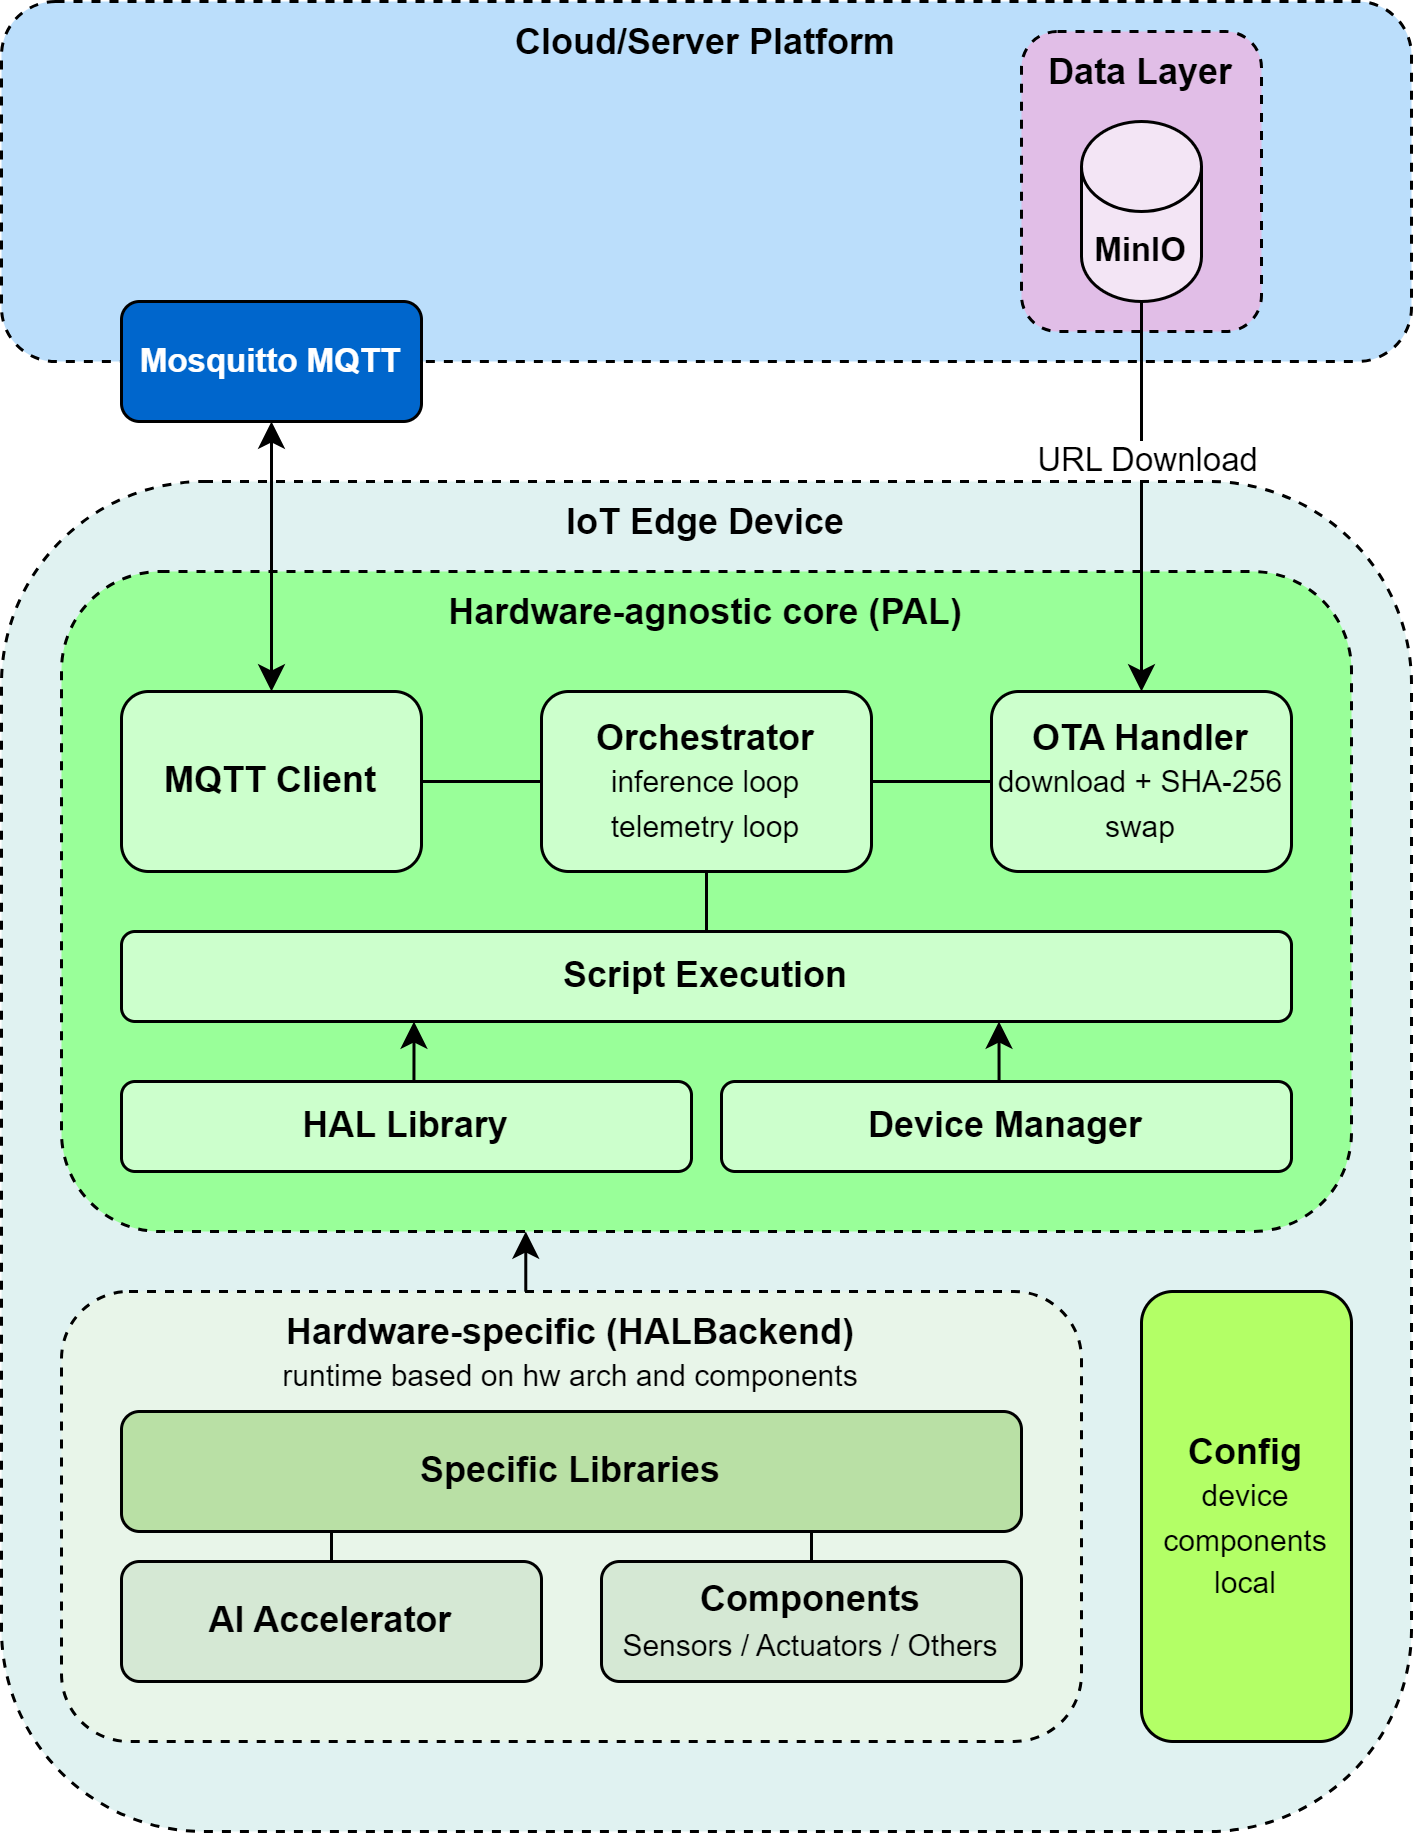
\includegraphics[width=0.75\linewidth]{images/IoT Edge Devices.png}
    \caption{\acrshort{IoT} Edge Devices Diagram}
    \label{fig:device_diagram}
\end{figure}

\subsubsection{Platform Abstraction Layer (\texorpdfstring{\acrshort{PAL}}{PAL})}\label{sec:impl:pal}

The \gls{PAL} serves as the hardware-agnostic core of the edge runtime, implemented as a modular Python service. It is containerized using Docker to run portably on various physical edge platforms. It is responsible for all inference coordination, device communication, model updates, and script execution, regardless of the underlying physical hardware. 

Its design isolates every hardware-dependent concern behind the \texttt{HALBackend} interface, described in \autoref{sec:impl:halbackend}, so that the components within the \gls{PAL} never reference hardware-specific code directly.

The \gls{PAL} is composed of six components: the \textbf{Orchestrator}, the \textbf{\gls{OTA} Handler}, the \textbf{\gls{MQTT} Client and Command Handler}, the \textbf{Device Manager}, the \textbf{Configuration Management}, and the \textbf{Script Runner}.

\subsubsection{Orchestrator}\label{sec:impl:orchestrator}

The Orchestrator is the central coordinator of the \gls{PAL}. It is implemented as an async Python class that launches three concurrent loops.
\begin{itemize}
    \item The \textbf{inference loop} reads frames from the active sensor through a \texttt{SensorManager}, preprocesses each frame through the active \texttt{HALBackend}, and runs inference. The result is then routed: if a custom script is loaded, the execution is passed to the \texttt{ScriptRunner} (which can execute logic before and after inference), returning a \texttt{TelemetryPayload}, otherwise the raw predictions are published directly. In both cases the output is published on \texttt{device/\{id\}/inference}.
    \item The \textbf{telemetry loop} publishes a system health snapshot to \texttt{device/\{id\}/telemetry} at the configured interval (default 10 seconds). This payload includes \gls{CPU} utilisation percentage (\texttt{cpu\_percent}), \gls{RAM} percentage (\texttt{ram\_percent}), \gls{RAM} used in MB (\texttt{ram\_used\_mb}), agent uptime in seconds (\texttt{uptime\_s}), the active deployment, model and script identifiers, physical sensor details, and system temperatures.
    \item The \textbf{liveness indicator} is embedded within this telemetry stream. Since the Edge Connector Service tracks the arrival of telemetry packets to update the device's \texttt{last\_seen\_at} timestamp in MongoDB, the telemetry loop effectively functions as a periodic heartbeat, eliminating the need for a separate concurrent thread.
\end{itemize}

\subsubsection{\texorpdfstring{\acrshort{OTA}}{OTA} Handler}\label{sec:impl:ota}

The \gls{OTA} Handler processes \texttt{ota\_update} commands received over \gls{MQTT}. The update sequence guarantees that the device always has a runnable model, even in the event of a corrupted download or a failed health check.

\begin{enumerate}
    \item \textbf{Download}: The compiled artefact is streamed from the presigned MinIO \gls{URL}. A progress event is published every 10\% of content length.
    \item \textbf{Verification}: The SHA-256 checksum of the downloaded file is computed incrementally and compared against the value in the command payload. A mismatch results in immediate failure without modifying the active model.
    \item \textbf{Backup}: The currently active model file is copied to a backup directory before any change is made.
    \item \textbf{Atomic swap}: The current model is replaced by the new downloaded one.
    \item \textbf{Health check}: The \texttt{\gls{HAL}Backend} reloads the model and executes a warmup pass. On failure, the backup is restored via an identical atomic swap and an \texttt{ota\_rolled\_back} event is published.
    \item \textbf{Completion}: An \texttt{ota\_completed} event is published. The Edge Connector Service receives it and transitions the deployment record to \textit{active}.
\end{enumerate}


\subsubsection{\texorpdfstring{\acrshort{MQTT}}{MQTT} Client and Command Handler}\label{sec:impl:mqtt_edge}

The \gls{MQTT} client connects to the platform broker on port 8883 with mutual \gls{TLS}: the device presents its client certificate signed by the platform \gls{CA}, and the broker verifies it before accepting the connection. If the connection is lost, the client retries automatically with a 10-second interval.

Incoming messages on \texttt{device/\{id\}/commands} are dispatched by a \texttt{CommandHandler} to the appropriate runtime component. Two command types are implemented:
\begin{itemize}
    \item \textbf{\texttt{deploy}}: Instructs the \gls{OTA} Handler to download a compiled model and custom script, verify their checksums, back up the previous model, and dynamically update the active deployment.
    \item \textbf{\texttt{update\_libraries}}: Commands the \gls{OTA} Handler to synchronize custom Python device libraries from the server when a hash mismatch is detected.
\end{itemize}

\subsubsection{Custom Scripts}\label{sec:impl:scripts}

Custom scripts allow operators to define custom processing logic that executes on the device before and after inference. This enables custom pre/post-processing and compound inference patterns without modifying the runtime codebase.

By contract, all scripts must contain exactly one implemented function:

\begin{center}
    \texttt{process(frames, results, context)} $\rightarrow$ \texttt{TelemetryPayload}
\end{center}

\begin{itemize}
    \item \texttt{frames} wraps the raw sensor numpy arrays.
    \item \texttt{results} carries the corresponding \texttt{HALBackend} outputs.
    \item \texttt{context} exposes read-only device metadata.
\end{itemize}

It returns an \texttt{InferenceResult}, which must be a \texttt{TelemetryPayload}: a structured object carrying an event name, a \gls{JSON}-serialisable data dictionary, a severity level (\textit{info}, \textit{warning}, \textit{alert}), and optional tags.

When a script is uploaded, it is analysed with Python's \texttt{ast} module before being stored. The \texttt{ScriptValidator} checks three conditions: the \texttt{process} function exists with exactly three parameters, all imports reference modules in the permitted whitelist, and no calls to forbidden built-ins appear anywhere in the syntax tree. Errors are returned as a structured list and displayed immediately in the frontend editor, before the user attempts to upload.

At runtime, the \texttt{ScriptRunner} loads the script source into a restricted global namespace containing only whitelisted module references and contract types, with a minimal \texttt{\_\_builtins\_\_} dictionary that excludes all filesystem, network, and subprocess access functions. 

The \texttt{process()} function is invoked in a daemon thread, the main event loop joins with the configured timeout. If the thread is still alive after the timeout, a \texttt{ScriptTimeoutError} is raised and the raw inference result is published as a fallback.

\subsubsection{Configuration Management}\label{sec:impl:config}

Device configuration is resolved at startup by merging four sources in decreasing priority order: environment variables (\texttt{DEVICE\_ID}, \texttt{MQTT\_HOST}, \texttt{MODEL\_ID}, etc.), \texttt{local.yaml} for operator-level overrides, \texttt{device.yaml} injected read-only by the platform at each deployment, and \texttt{peripherals.yaml} listing the physical peripherals attached to the device. The merged result is exposed as a module-level singleton throughout the runtime, so all components share a single consistent configuration without repeated file \gls{IO}.

\subsubsection{Device Manager}\label{sec:impl:device_manager}

The \texttt{DeviceManager} acts as the hardware resource manager, responsible for reading the peripheral layout from the YAML configuration, instantiating the appropriate device backends for each enabled component, and handling their lifecycle. During system startup, it instantiates the registered device wrapper classes and opens their communication channels. 

Throughout the runtime, the \texttt{DeviceManager} provides a unified, keyed-access interface that allows the Orchestrator to interact with specific peripherals (such as cameras) without coupling the core logic to the underlying concrete drivers. When the runtime shuts down, it handles the orderly closure of all active hardware backends.


\subsubsection{Hardware Abstraction Layer (\texorpdfstring{\acrshort{HAL}}{HAL}) Backend}\label{sec:impl:halbackend}

The \gls{HAL}Backend is designed as a hardware-independent boundary layer that decouples the \gls{PAL} from specific physical hardware platforms and peripherals. It exposes generic high-level functions (such as executing model inference or capturing images) to the \gls{PAL} Orchestrator, while dynamically delegating these calls to concrete device backends based on the runtime configuration. The abstraction is split into two primary interfaces.

\paragraph{Inference \gls{HAL}Backend}
The inference engine is managed through the \texttt{HALBackend} abstract class, exposing three main methods:

\begin{itemize}
    \item \textbf{\texttt{load\_model(path)}}: Loads the compiled model binary into the device memory or hardware accelerator.
    \item \textbf{\texttt{preprocess(raw\_frame)}}: Converts raw sensor frames into the tensor format expected by the model.
    \item \textbf{\texttt{infer(input\_data)} $\rightarrow$ \texttt{InferenceResult}}: Executes a single forward pass and returns bounding box predictions.
\end{itemize}

The active inference backend is resolved at startup by checking the \texttt{hardware\_arch} field in the configuration and in
stantiating the corresponding wrapper. Four built-in implementations are supported:
\todo{actualizar hw}
\begin{itemize}
    \item \textbf{Hailo Backend}: Interfaces with the HailoRT library to load \texttt{.hef} binaries into Hailo-8/8L accelerators.
    \item \textbf{IMX500 Backend}: Connects to the Sony IMX500 AI Camera drivers to execute packed models directly on-sensor.
    \item \textbf{TensorRT Backend}: Utilizes NVIDIA's TensorRT runtime engine with CUDA support on Jetson platforms.
    \item \textbf{TFLite Backend}: Employs the TensorFlow Lite Interpreter as a fallback for general CPU architectures.
\end{itemize}

\paragraph{Peripheral \gls{HAL}Backend}
Peripherals are managed via the \texttt{DeviceManager}, which reads the active device layout from \texttt{components\_config.yaml} at startup. When the \gls{PAL} requests a generic action, such as capturing a frame, the \texttt{DeviceManager} routes the request to the designated backend:

\begin{itemize}
    \item \textbf{Built-in Drivers}: Standard implementations for generic hardware (e.g., \texttt{opencv} or \texttt{libcamera} for cameras).
    \item \textbf{Dynamic Drivers}: Custom user-defined drivers located in the dynamic \texttt{hardware/} folder (e.g., \texttt{hardware/sensors/camera/<driver>/library.py}).
\end{itemize}

This decoupling enables a generic execution flow. For instance, when the Orchestrator initiates a camera frame capture:

\begin{enumerate}
    \item The Orchestrator calls the generic \texttt{capture\_frame()} method on the configured camera instance.
    \item The dynamically loaded generic wrapper (e.g., defined in \texttt{hardware/sensors/camera/generic.py}) checks the active configuration. If a \gls{RPi} Camera Module 3 is active (\texttt{rpi\_camera\_module\_3}), it loads the corresponding custom library module dynamically.
    \item The generic call is delegated to the specific implementation (e.g., invoking \texttt{read\_value()} within the \texttt{RPiCameraLibrary} class).
\end{enumerate}

This ensures that adding new physical devices or switching active peripherals requires only updating the configuration files and providing the corresponding driver script, without recompiling or altering the core \gls{PAL} codebase.

\subsection{Dynamic Hardware Registry and Auto-Synchronisation}\label{sec:impl:dyn_hardware}

To enable seamless extensibility without modifying the core backend services or the edge runtime codebase, the platform implements a dynamic discovery and hot-reload system for hardware architectures, sensors, actuators, and other auxiliary modules. All hardware-specific definition files are unified under a shared \texttt{hardware/} directory \footnote{For this \gls{PoC}, Python is the only language used. In reality, it would be several copies of that file but in different languages such as C++ or Java.}.

\begin{figure}[H]
    \centering
    \begin{minipage}{0.48\textwidth}
        \centering
        \textbf{Server-Side Compilation Module}
        \begin{verbatim}
    hardware/
    └── hw_arch/
        └── <arch_name>/
            └── compilation/
                └── compiler.py
        \end{verbatim}
    \end{minipage}
    \hfill
    \begin{minipage}{0.48\textwidth}
        \centering
        \textbf{Edge-Side Inference Module}
        \begin{verbatim}
    hardware/
    └── hw_arch/
        └── <arch_name>/
            └── inference/
                └── library.py
        \end{verbatim}
    \end{minipage}
    \caption{Dynamic Hardware Architecture Directory Layout}
    \label{fig:hw_arch_layout}
\end{figure}

\begin{figure}[H]
    \centering
    \begin{minipage}{0.23\textwidth}
        \centering
        \textbf{Sensors Module}
        \begin{verbatim}
hardware/
└── sensors/
    └── <category>/
        └── <sensor_name>/
        \end{verbatim}
    \end{minipage}
    \hfill
    \begin{minipage}{0.23\textwidth}
        \centering
        \textbf{Actuators Module}
        \begin{verbatim}
hardware/
└── actuators/
    └── <category>/
        └── <actuator_name>/
        \end{verbatim}
    \end{minipage}
    \hfill
    \begin{minipage}{0.23\textwidth}
        \centering
        \textbf{Others Module}
        \begin{verbatim}
hardware/
└── others/
    └── <category>/
        └── <other_name>/
        \end{verbatim}
    \end{minipage}
    \caption{Dynamic Peripherals Directory Layout}
    \label{fig:peripherals_layout}
\end{figure}

The extensibility mechanism is based on three main operational concepts:

\begin{itemize}
    \item \textbf{Structured Layout}: New hardware architectures and peripherals are introduced by creating subdirectories under \texttt{hardware/hw\_arch/<arch\_name>/} or the corresponding category subfolders (\texttt{sensors}, \texttt{actuators}, \texttt{others}), as shown in \autoref{fig:hw_arch_layout} and \autoref{fig:peripherals_layout}. 
    
    Hardware architectures separate compilation logic (\texttt{compilation/compiler.py}) and inference drivers (\texttt{inference/library.py}). Peripherals contain a single \texttt{library.py} specifying their configuration and driver class. All modules must define a global \texttt{LABEL} variable for \gls{UI} cataloging.
    
    \item \textbf{Static Discovery via \gls{AST}}: To discover human-readable labels and register catalog entries without executing untrusted Python code, the \gls{MLOps} Service statically parses target files using Python's \texttt{ast} module. It extracts the top-level \texttt{LABEL} assignment safely and efficiently.
    
    \item \textbf{Dynamic Loading at Runtime}: At execution time, both the edge runtime and the server-side services dynamically load these modules using Python's \texttt{importlib.util} and \texttt{inspect} modules.
    
    To achieve total decoupling and avoid hardcoding peripheral categories, the generic category-level classes (e.g. cameras) are themselves defined within the \texttt{hardware/} directory (e.g., \texttt{hardware/sensors/camera/generic.py}). 
    
    These generic wrappers expose a standardized \gls{API} to the \gls{PAL} Orchestrator, but resolve the active peripheral configuration dynamically at startup to import and delegate calls  to the corresponding specific library (e.g., \texttt{hardware/sensors/camera/rpi\_camera\_module\_3/library.py}).
    
    This design allows adding completely new categories of peripherals without modifying a single line of the core edge runtime code.
\end{itemize}

\subsubsection{Dynamic Checksum Verification and \acrshort{OTA} Library Sync}\label{sec:impl:dyn_hardware:sync}

The synchronisation of these driver directories between the server-side platform and the edge set is coordinated via a dynamic checksum verification protocol. The sequence proceeds as follows:

\begin{enumerate}
    \item \textbf{Deterministic Hash Generation}: The relative paths and binary file contents are incrementally hashed using the SHA-256 algorithm to output a single representative hash string. To ensure repeatability, subdirectories and files are sorted lexicographically, and files such as \texttt{\_\_pycache\_\_} are ignored.
    
    \item \textbf{Telemetry Verification Loop}: The edge device publishes its current \texttt{libraries\_hash} inside its periodic telemetry heartbeat payload over \gls{MQTT}. The Edge Connector Service receives this payload, computes the platform's local checksum, and compares the two hash strings.
    
    \item \textbf{Dynamic Sync Command}: If a checksum mismatch is observed:
    \begin{enumerate}
        \item The Edge Connector packages the server's local \texttt{hardware/} directory into a memory-buffered ZIP archive and uploads it to the \texttt{compiled} bucket in MinIO.
        \item It publishes an \texttt{update\_libraries} command to the \gls{MQTT} topic \texttt{device/\{id\}/commands}, carrying the presigned MinIO \gls{URL} of the ZIP archive and the expected SHA-256 hash.
    \end{enumerate}
    
    \item \textbf{Atomic Swap on Edge Device}: Upon receiving the command, the edge \gls{OTA} Handler downloads the ZIP archive, validates its SHA-256 integrity, deletes all existing local subdirectories to prevent stale file conflicts, extracts the ZIP archive into the runtime hardware directory, and publishes an acknowledgment. 
    
    The \gls{PAL} Orchestrator then reloads the dynamically imported modules, immediately activating the new drivers without requiring a container rebuild or a system restart.
\end{enumerate}




